\chapter[Dados de ocorrência]{Dados de ocorrência, limpeza espacial e preparação de registros}

\begin{objetivos}
	Ao final desta unidade, o estudante deverá ser capaz de compreender as principais fontes de dados de ocorrência utilizadas em Modelagem de Distribuição de Espécies; reconhecer limitações associadas a dados de herbários, inventários e repositórios globais; padronizar registros taxonômicos e geográficos; filtrar ocorrências pelo limite do bioma Amazônia; remover coordenadas problemáticas, duplicatas e registros espacialmente redundantes; aplicar rarefação espacial; extrair variáveis ambientais associadas às ocorrências; e preparar uma base final de registros para as unidades posteriores de modelagem.
\end{objetivos}

\section{Introdução}

Dados de ocorrência constituem a base empírica da Modelagem de Distribuição de Espécies. Em modelos correlativos, os registros geográficos da espécie são associados às condições ambientais dos locais onde ela foi observada, permitindo estimar relações entre ocorrência e ambiente. Entretanto, a qualidade dos modelos depende diretamente da qualidade desses registros.

Em aplicações reais, os dados de ocorrência podem ser obtidos de inventários florestais, herbários, coleções biológicas, plataformas digitais, literatura científica e repositórios globais como o GBIF. Esses dados frequentemente combinam diferentes níveis de precisão taxonômica, geográfica e temporal. Por isso, antes da modelagem, é necessário realizar uma etapa cuidadosa de padronização, limpeza e filtragem espacial \parencite{guisan2017habitat,hijmans2021species,zizka2019coordinatecleaner}.

\begin{conceito}[title={\faBook\quad Registro de ocorrência}]
	Um registro de ocorrência é uma evidência espacial da presença de uma espécie em determinado local. Em SDM, esse registro normalmente é representado por coordenadas geográficas associadas ao nome da espécie, fonte do dado e, quando disponível, data, instituição, coletor e precisão espacial.
\end{conceito}

\section{Fontes de dados de ocorrência}

Os dados usados em SDM podem vir de diferentes fontes. Inventários florestais geralmente apresentam maior controle taxonômico e espacial, mas tendem a cobrir áreas limitadas. Herbários e coleções biológicas fornecem registros históricos valiosos, porém podem conter coordenadas imprecisas ou ausentes. Plataformas globais, como GBIF, ampliam a cobertura espacial, mas exigem filtros rigorosos de qualidade.

No estudo de referência usado nesta apostila, os registros de \textit{Dinizia excelsa} foram integrados a dados de inventário e GBIF, e posteriormente submetidos a filtros espaciais, rarefação e extração de variáveis bioclimáticas para análise de nicho climático na escala amazônica \parencite{delima2026warmer}. Esse fluxo é semelhante ao que será implementado nesta unidade.

\begin{dica}[title={\faLightbulb\quad Integração de fontes}]
	Uma boa base de ocorrência pode combinar inventários, herbários e GBIF, desde que todos os registros passem por padronização, limpeza e controle de duplicatas.
\end{dica}

\section{Problemas comuns em dados de ocorrência}

Os problemas mais frequentes incluem nomes científicos inconsistentes, coordenadas inválidas, registros no oceano, pontos em capitais, coordenadas de instituições, duplicatas, inversão de latitude e longitude, erros de georreferenciamento e forte viés espacial de amostragem.

Em espécies amazônicas, é comum haver concentração de registros próximos a rios, estradas, cidades, herbários, áreas de inventário e regiões de maior acesso logístico. Esse padrão não representa necessariamente maior adequabilidade ambiental, mas sim maior esforço de coleta.

\begin{atencao}[title={\faExclamationTriangle\quad Ocorrência não é ausência}]
	Registros de presença indicam onde a espécie foi observada. A ausência de registros em uma região não significa necessariamente ausência da espécie; pode refletir ausência de amostragem.
\end{atencao}

\section{Fluxo de preparação dos dados}

O fluxo usado nesta unidade segue a lógica geral de estudos de SDM em escala amazônica: compilação dos registros, padronização de colunas, filtragem por coordenadas válidas, correção espacial, recorte pelo bioma, remoção de duplicatas, rarefação espacial, extração ambiental e exportação da base final.

\rscriptfile{scripts/unidade02/01_compilar_ocorrencias_dinizia.R}

\section{Limpeza geográfica e recorte pelo bioma Amazônia}

Após a compilação, os registros são convertidos para objetos espaciais, avaliados quanto à validade das coordenadas e filtrados pelo limite do bioma Amazônia. Essa etapa garante que a base de trabalho represente a escala geográfica definida para o estudo.

\rscriptfile{scripts/unidade02/02_limpeza_espacial_dinizia.R}

\begin{figure}[H]
	\centering
	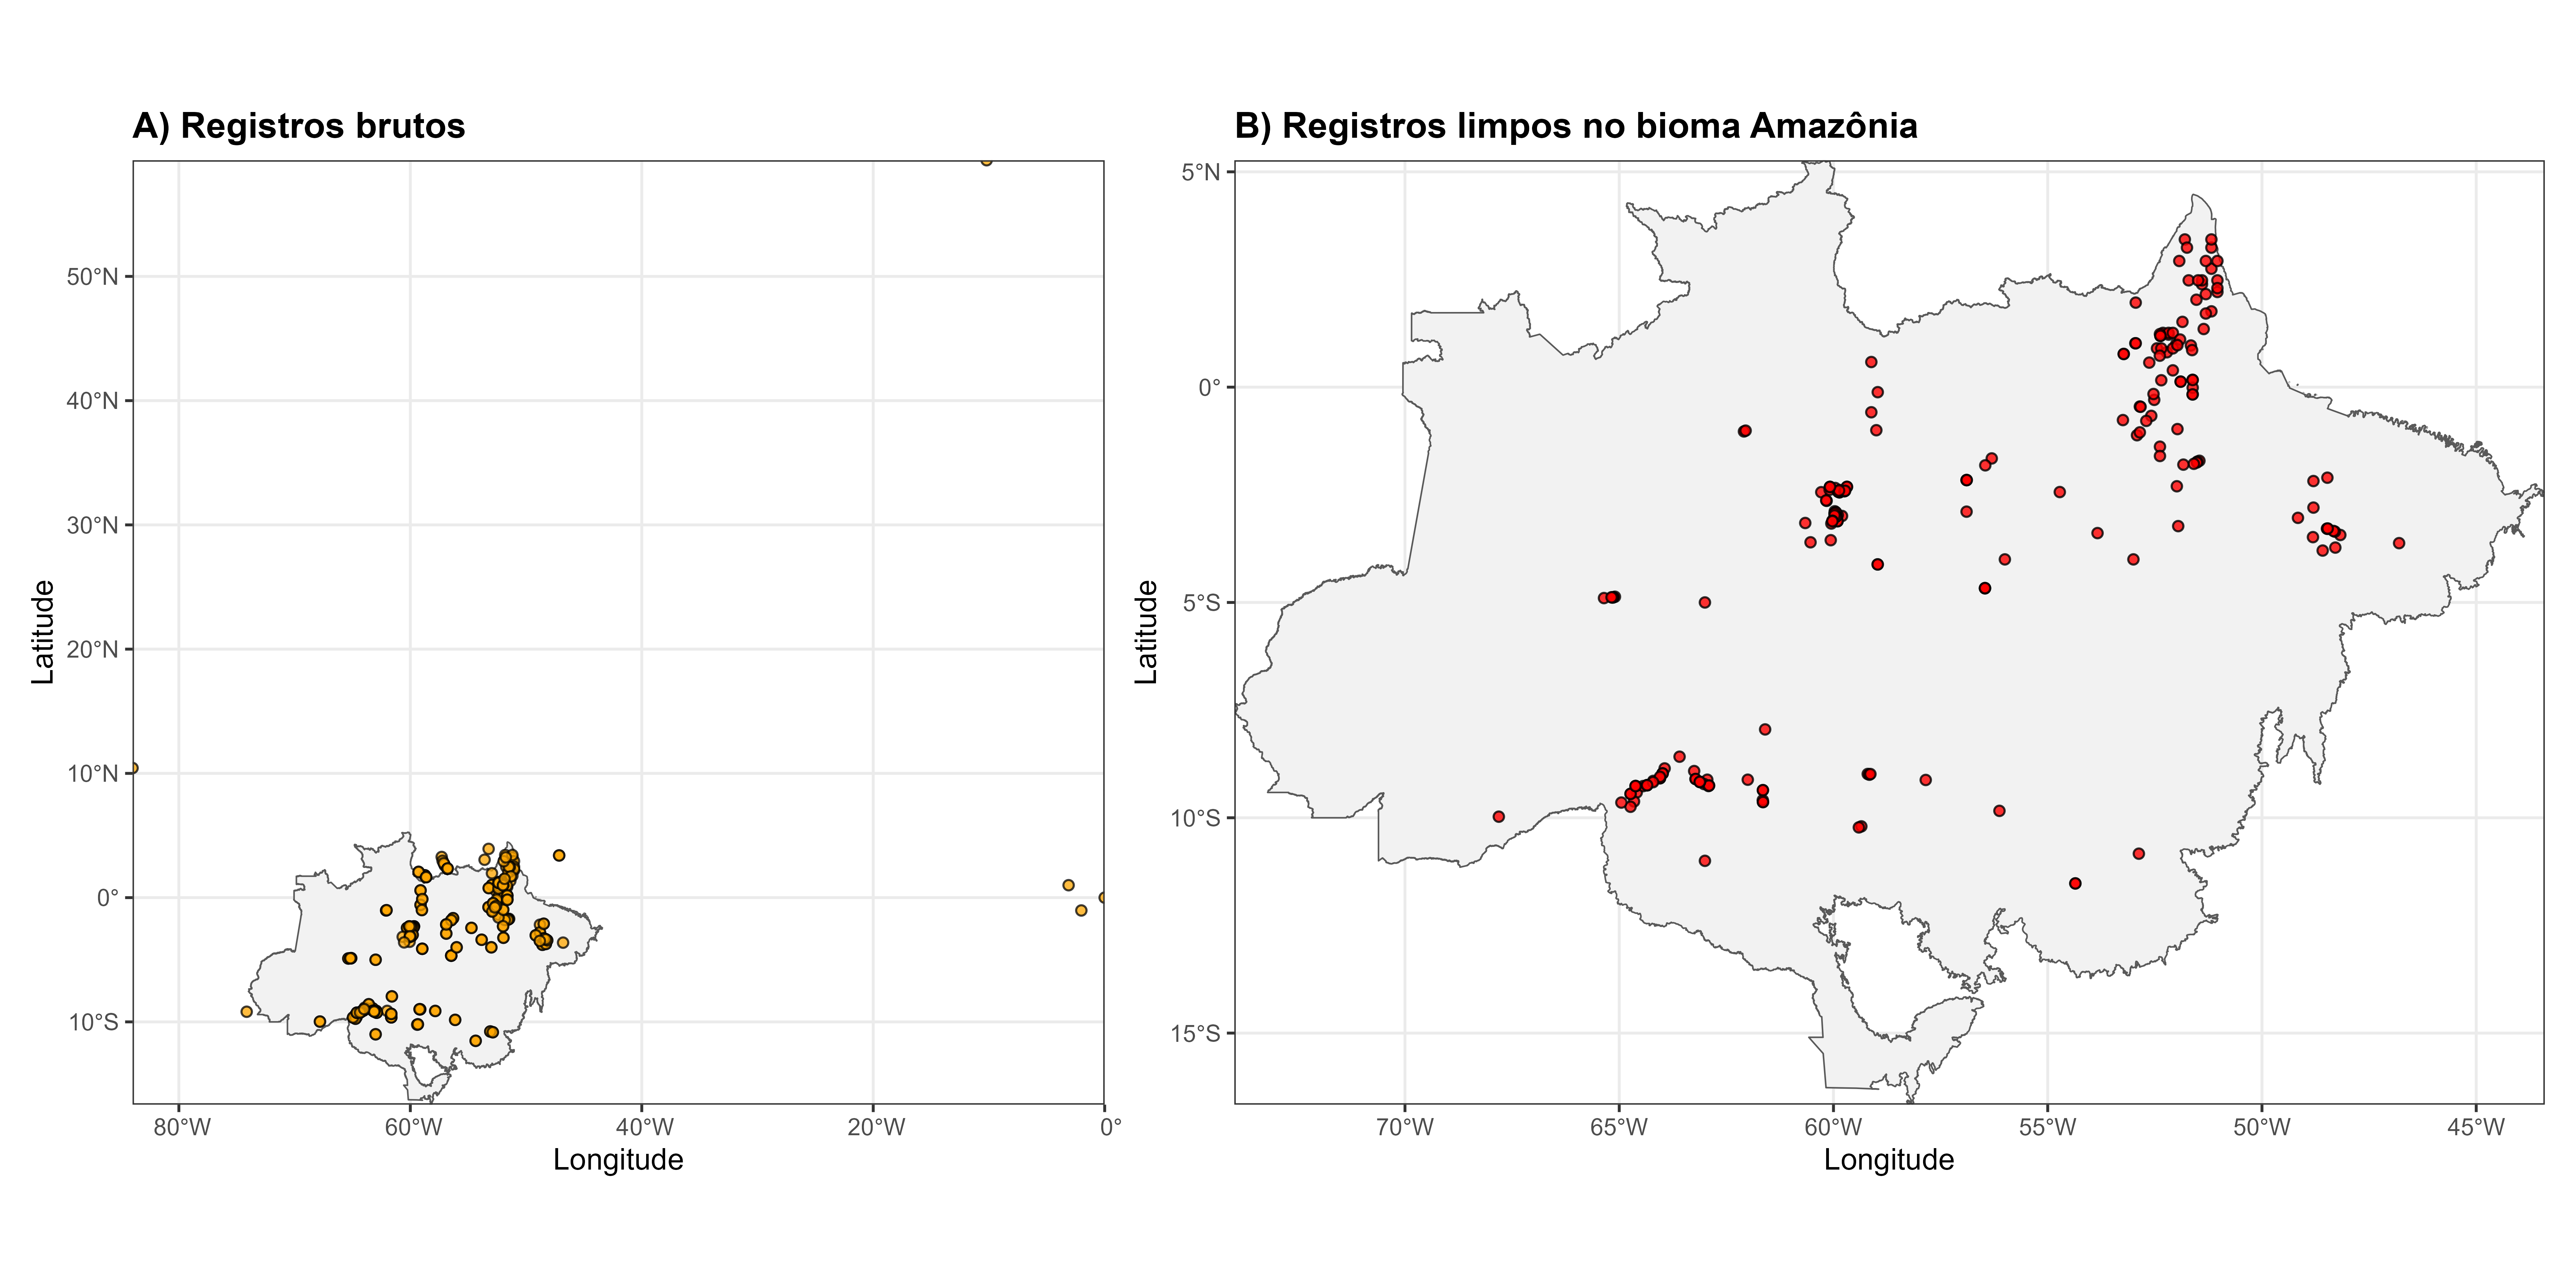
\includegraphics[width=0.92\textwidth]{figuras/unidade02/unidade02_mapa_bruto_limpo_dinizia.png}
	\caption{Comparação entre registros brutos e registros filtrados de \textit{Dinizia excelsa} no bioma Amazônia.}
	\label{fig:unidade02_bruto_limpo_dinizia}
\end{figure}

\section{Extração ambiental e duplicatas por célula raster}

Mesmo após remover coordenadas idênticas, diferentes registros podem cair no mesmo pixel climático. Como os modelos usam valores ambientais extraídos de rasters, múltiplos pontos no mesmo pixel podem representar pseudorreplicação ambiental. Por isso, é recomendável remover duplicatas por célula raster, mantendo apenas um registro por pixel ambiental.

\rscriptfile{scripts/unidade02/03_extrair_ambiente_dinizia.R}

\section{Rarefação espacial}

A rarefação espacial reduz a concentração excessiva de registros em áreas muito amostradas. Nesta unidade, aplicamos uma distância mínima entre ocorrências, permitindo reduzir autocorrelação espacial e viés de amostragem. Esse procedimento é amplamente usado em estudos de nicho ecológico e pode ser implementado com o pacote \texttt{spThin} \parencite{aiellolammens2015spthin}.

\rscriptfile{scripts/unidade02/04_rarefacao_espacial_dinizia.R}

\begin{figure}[H]
	\centering
	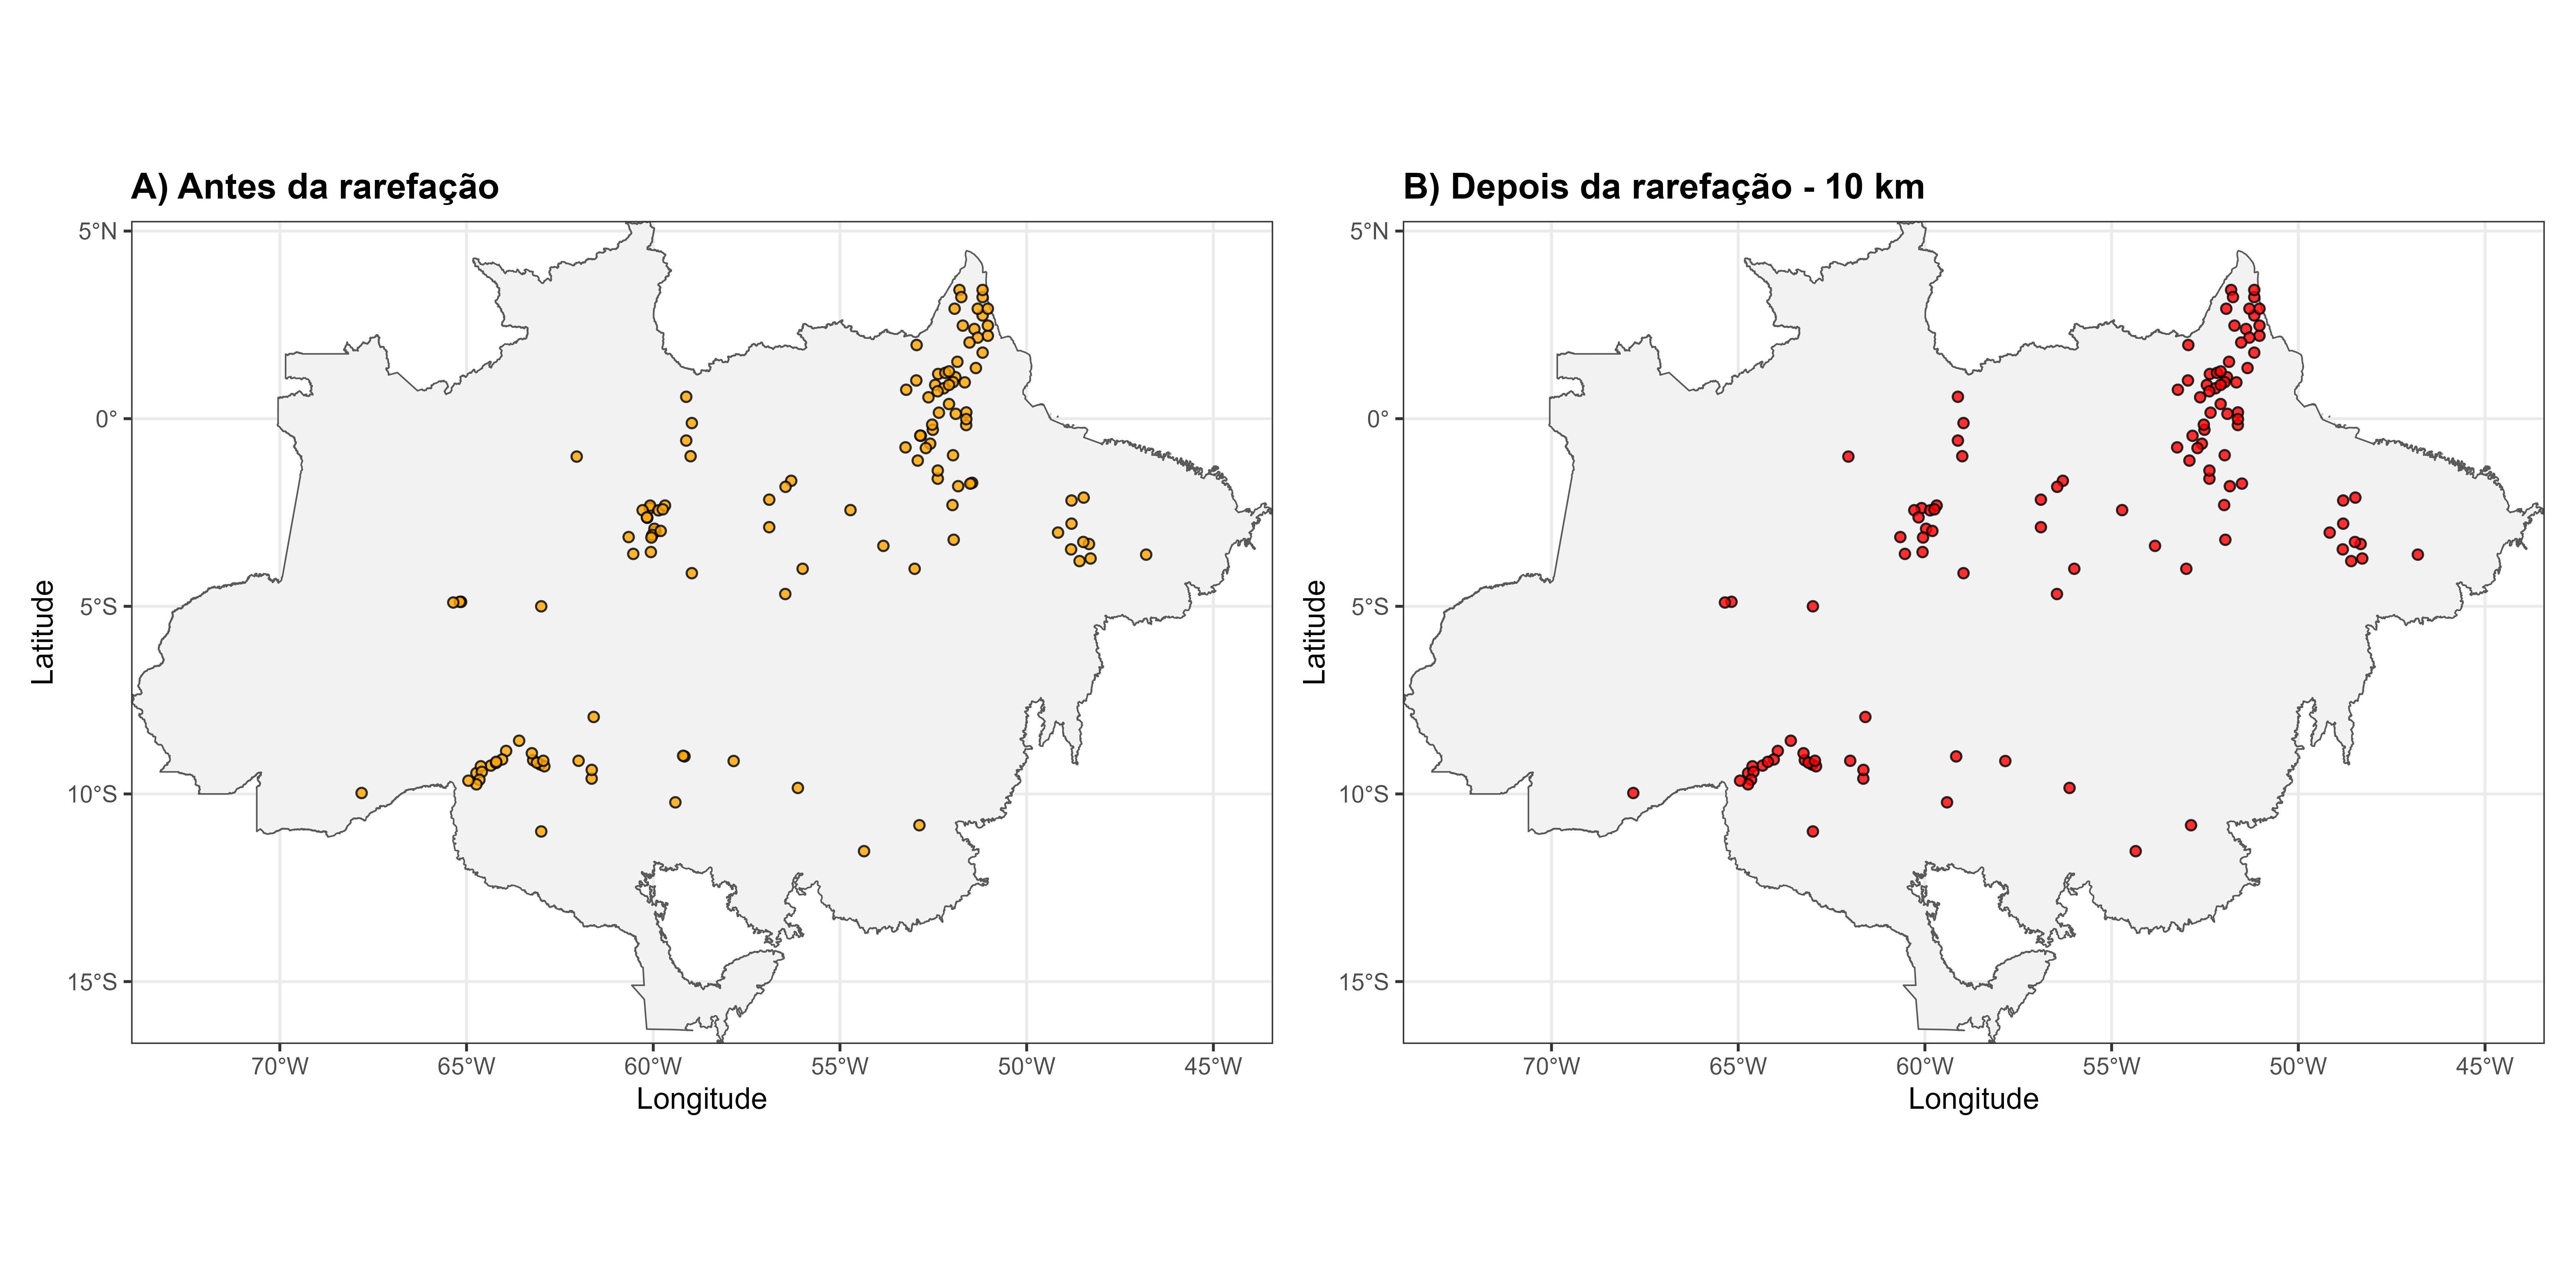
\includegraphics[width=0.92\textwidth]{figuras/unidade02/unidade02_rarefacao_dinizia.png}
	\caption{Efeito da rarefação espacial nos registros de \textit{Dinizia excelsa}. O procedimento reduz a redundância espacial e a concentração de pontos próximos.}
	\label{fig:unidade02_rarefacao_dinizia}
\end{figure}

\section{Diagnóstico ambiental dos registros}

Após a limpeza e rarefação, as ocorrências finais são associadas às variáveis ambientais selecionadas. Essa etapa permite verificar a amplitude climática ocupada pela espécie, identificar valores extremos e preparar a matriz final para modelagem.

\rscriptfile{scripts/unidade02/05_diagnostico_ambiental_dinizia.R}

\begin{figure}[H]
	\centering
	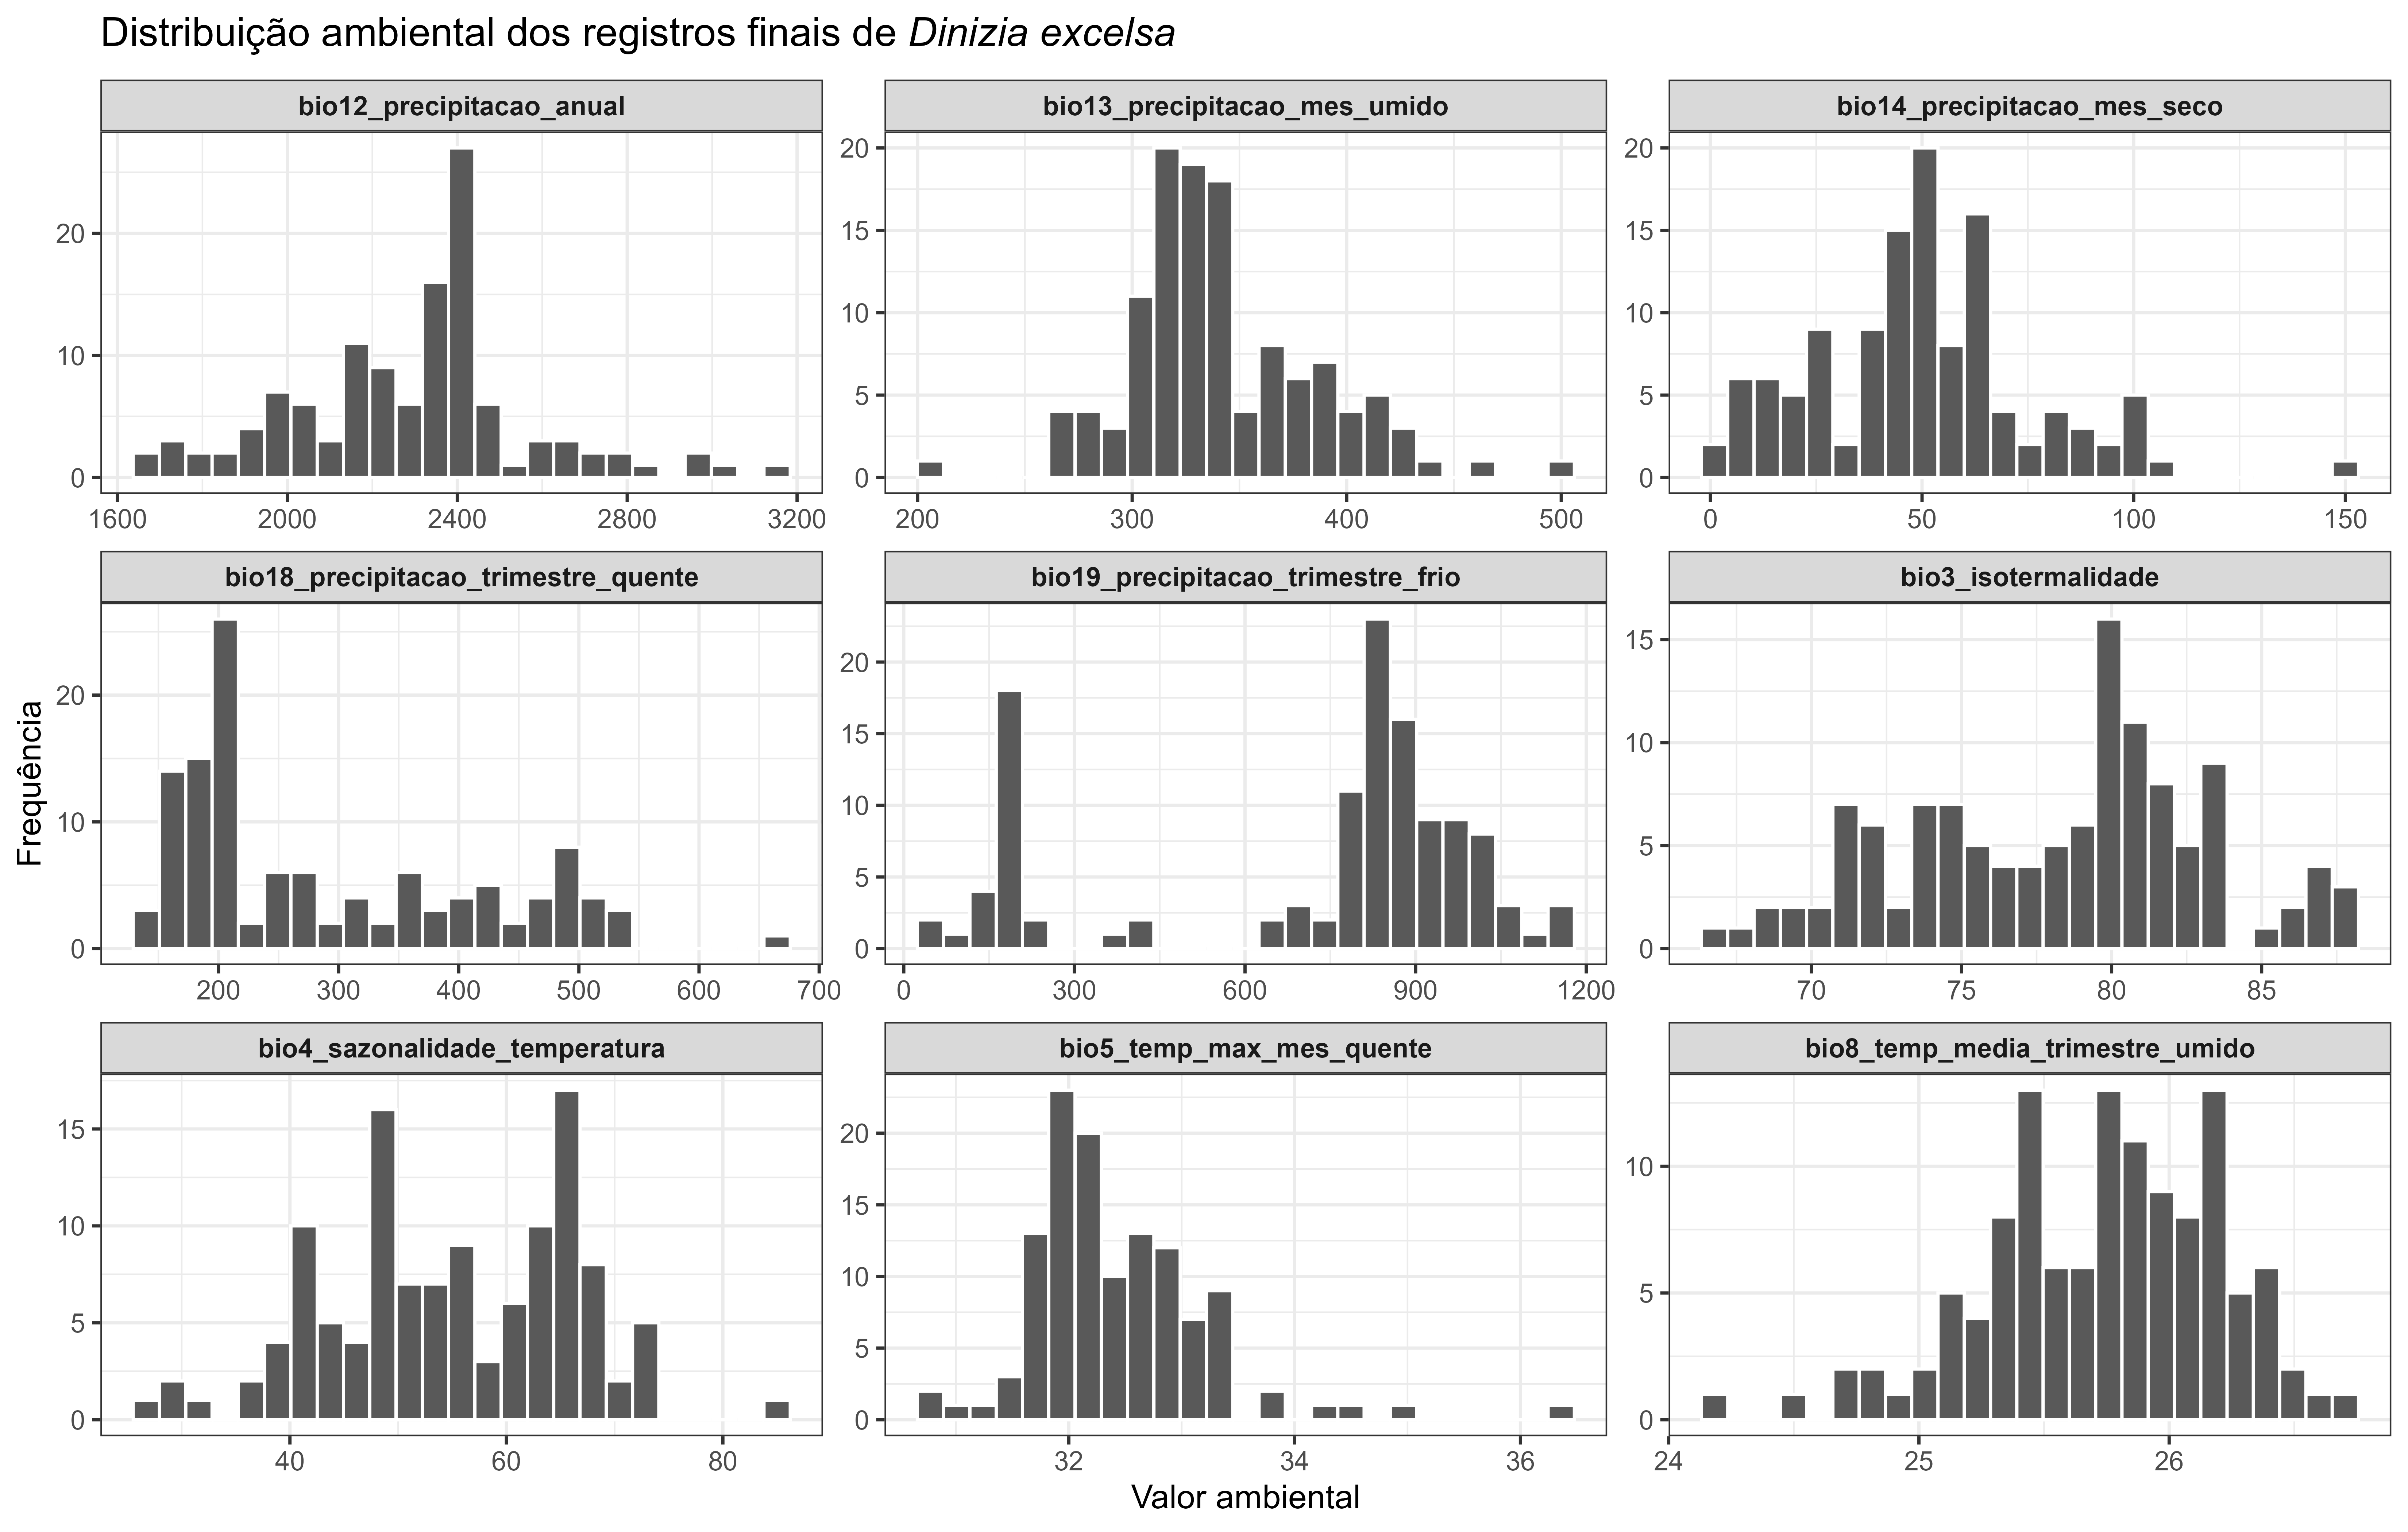
\includegraphics[width=0.92\textwidth]{figuras/unidade02/unidade02_histogramas_variaveis_dinizia.png}
	\caption{Distribuição das variáveis bioclimáticas extraídas nos registros finais de \textit{Dinizia excelsa}.}
	\label{fig:unidade02_hist_variaveis_dinizia}
\end{figure}

\begin{figure}[H]
	\centering
	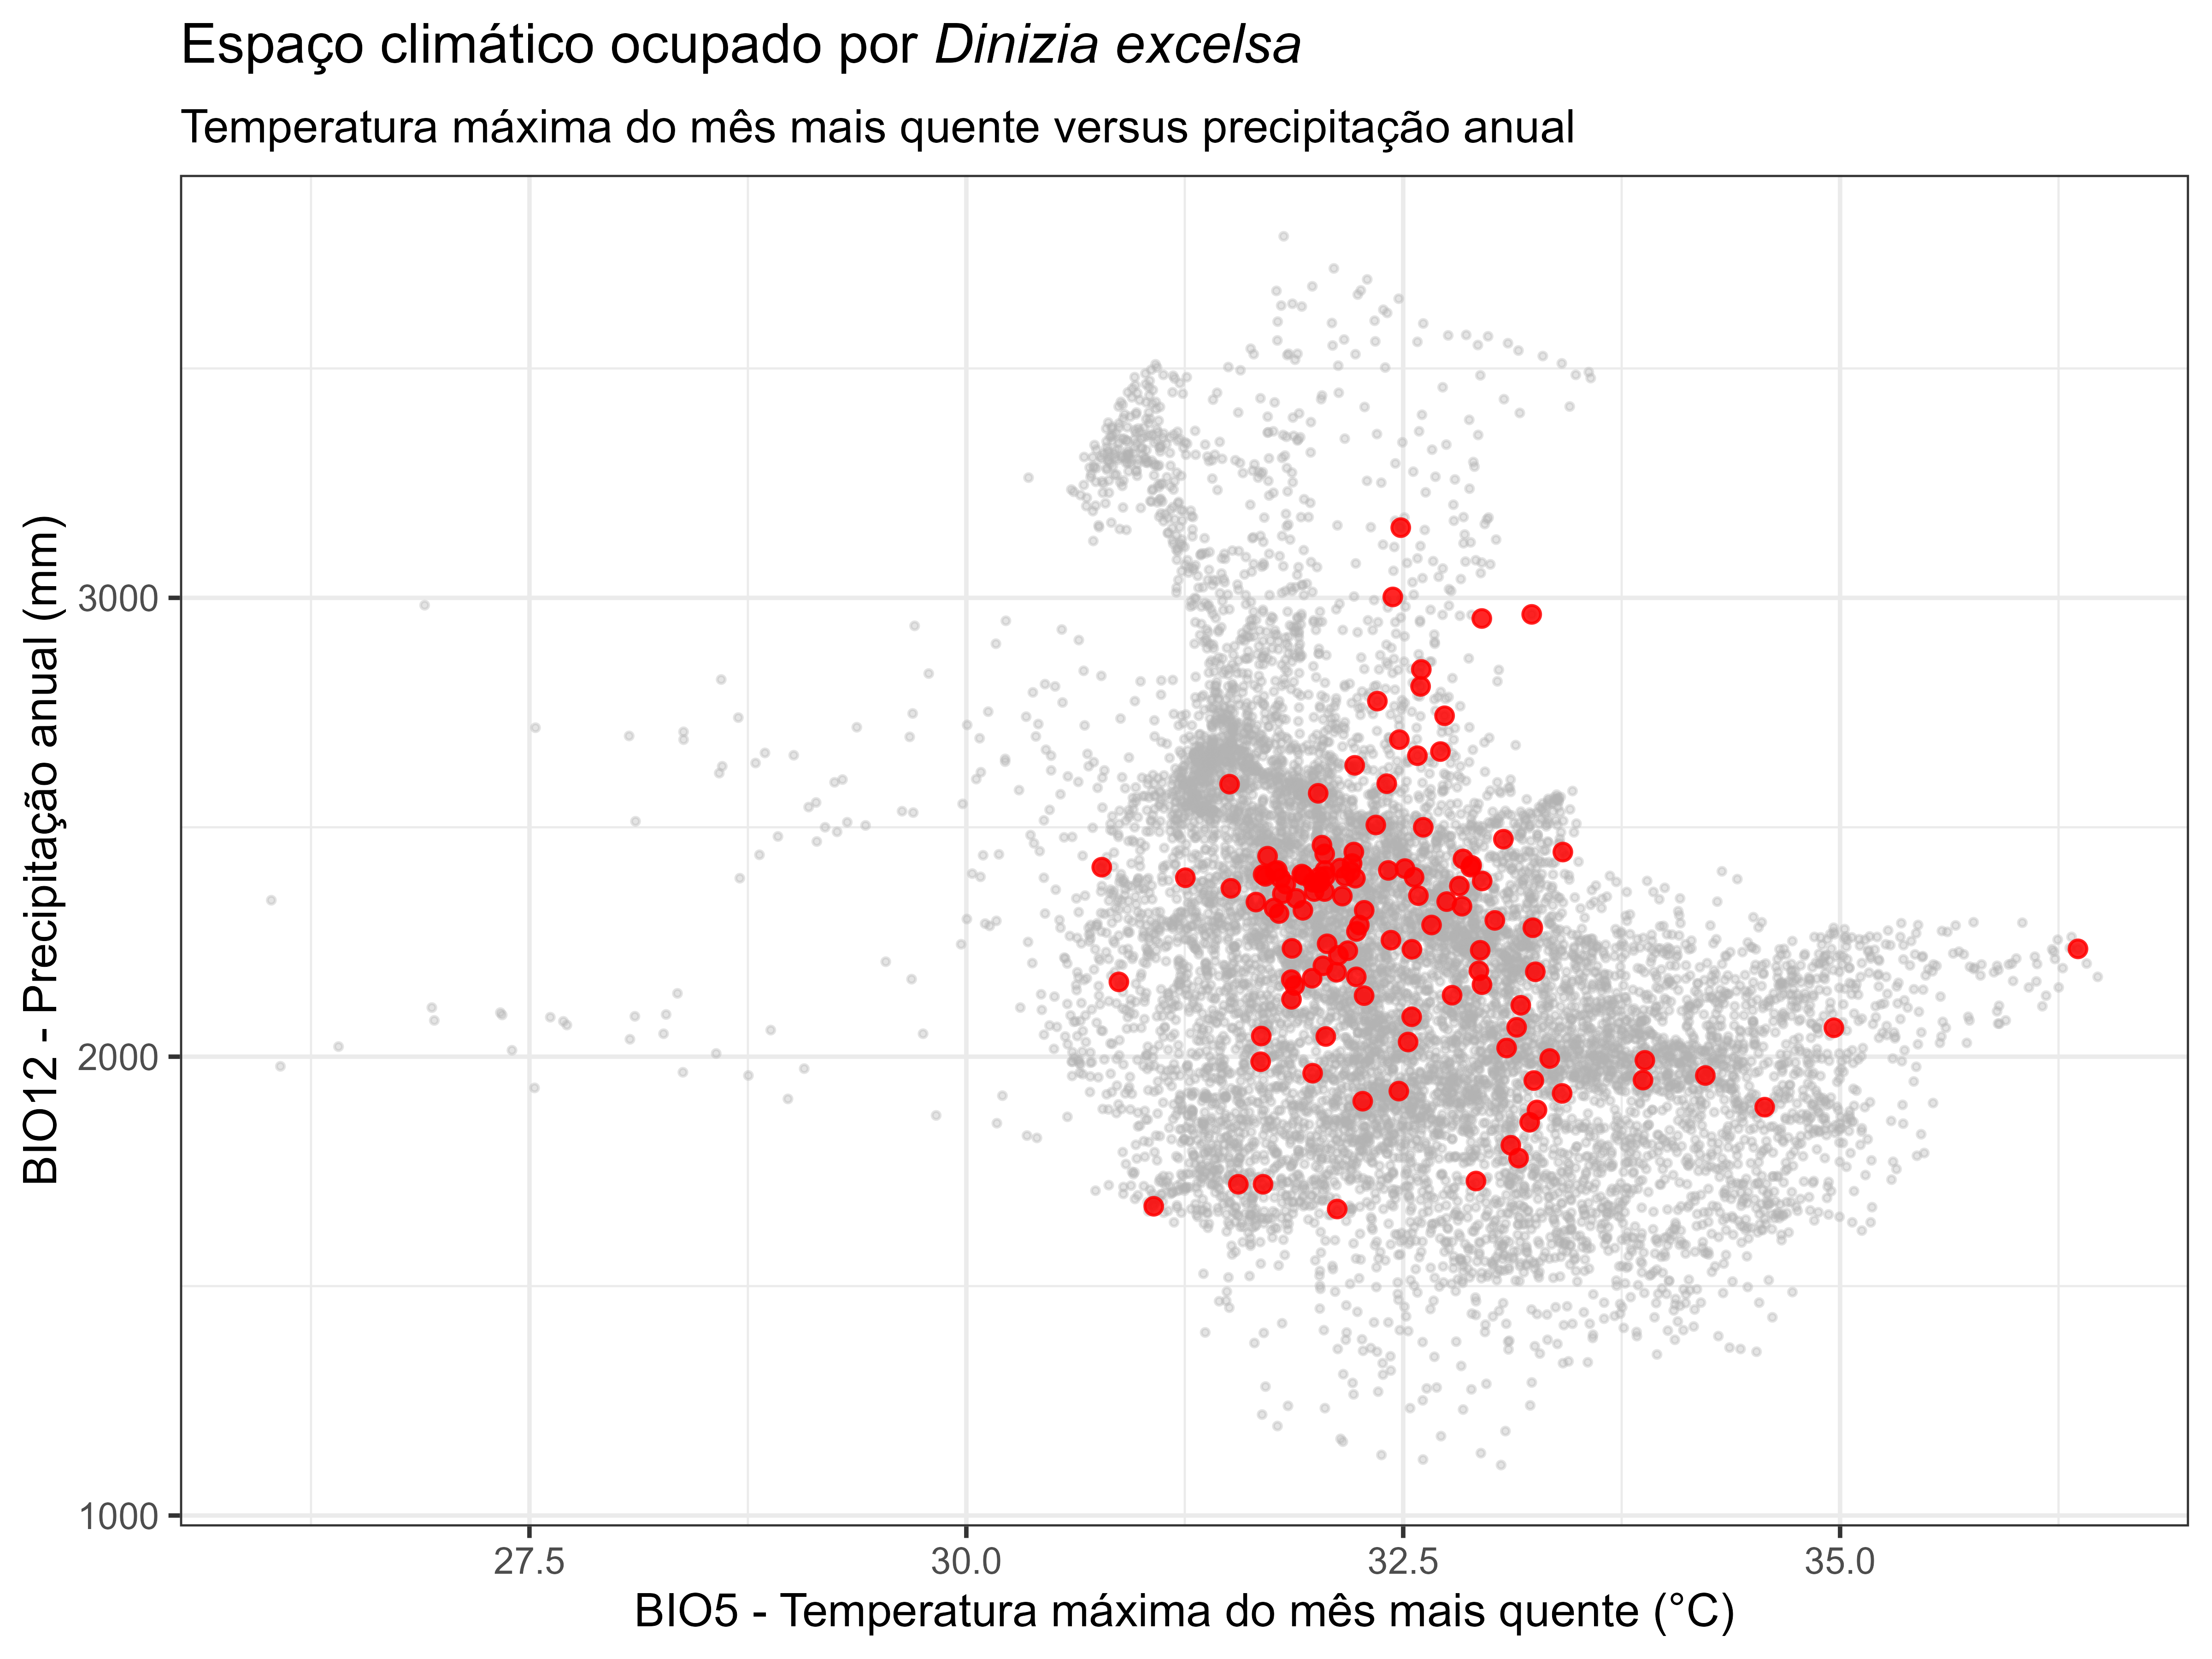
\includegraphics[width=0.86\textwidth]{figuras/unidade02/unidade02_espaco_climatico_dinizia.png}
	\caption{Espaço climático ocupado por \textit{Dinizia excelsa} em relação ao background ambiental do bioma Amazônia.}
	\label{fig:unidade02_espaco_climatico_dinizia}
\end{figure}

\section{Fluxograma do processamento}

O fluxograma resume a sequência de decisões adotadas para transformar registros brutos em uma base final de modelagem.

\rscriptfile{scripts/unidade02/06_fluxograma_preparacao_dinizia.R}

\begin{figure}[H]
	\centering
	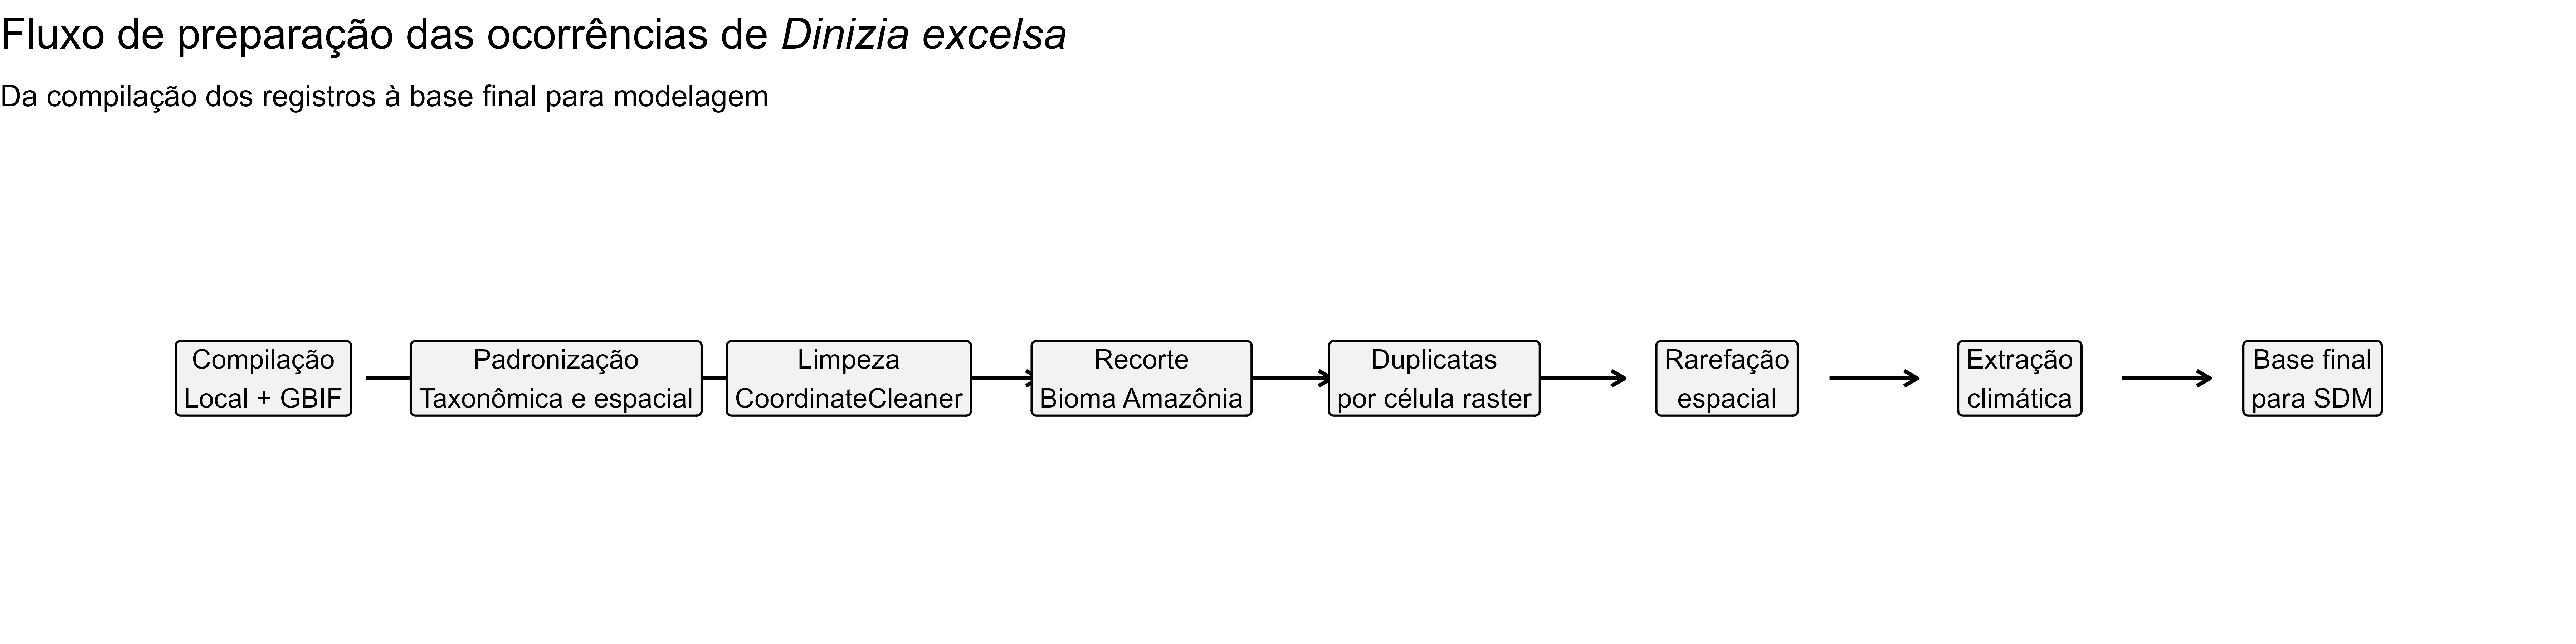
\includegraphics[width=0.92\textwidth]{figuras/unidade02/unidade02_fluxograma_preparacao_dinizia.png}
	\caption{Fluxograma de preparação de dados de ocorrência para SDM usando \textit{Dinizia excelsa} como estudo de caso.}
	\label{fig:unidade02_fluxograma_dinizia}
\end{figure}

\section{Pipeline completo da Unidade 2}

\rscriptfile{scripts/unidade02/07_pipeline_unidade02_dinizia.R}

\section{Síntese da unidade}

A preparação dos dados de ocorrência é uma das etapas mais importantes da SDM. Modelos sofisticados não corrigem dados ruins. A qualidade final da modelagem depende da coerência taxonômica, validade espacial, controle de duplicatas, redução de viés amostral e compatibilidade entre registros e variáveis ambientais.

\begin{conceito}[title={\faBook\quad Mensagem central}]
	Antes de ajustar qualquer algoritmo, é necessário transformar registros brutos em uma base de ocorrência limpa, espacialmente coerente, ambientalmente consistente e compatível com a escala do estudo.
\end{conceito}

\section{Exercícios de fixação}

\begin{enumerate}
	\item Explique por que registros de GBIF e herbários precisam ser limpos antes da modelagem.
	\item Diferencie duplicata geográfica e duplicata por célula raster.
	\item Por que registros fora do bioma de estudo devem ser removidos?
	\item Explique a finalidade da rarefação espacial.
	\item O que é viés de amostragem em SDM?
	\item Por que a ausência de registros não deve ser interpretada automaticamente como ausência da espécie?
	\item Proponha um fluxo de limpeza para uma espécie arbórea amazônica rara.
\end{enumerate}

% ============================================================
% UNIDADE 3
% ============================================================

